\section{Task 3: Spending compute at test time}
\label{sec:task3}

The test-time study uses supplied pools of 32 sampled solutions (rollouts) per question, from Qwen2.5-3B-Instruct on 1,000 MATH problems and Qwen2.5-VL-3B-Instruct on 1,000 MathVista problems; we report the 800 evaluation questions of each seeded split. Answers are grouped by equivalence without consulting the gold answer, and missing answers form one NO\_ANSWER group that is always wrong. For each budget $N$ from 1 to 32, every selection rule sees the same first $N$ rollouts of ten seeded orders, and cost counts the generated tokens consumed. Apart from majority voting (self-consistency), rollouts are scored by mean token log-probability $L$, self-certainty~\citep{kang2025selfcertainty} $K$ (the mean KL divergence of each next-token distribution from uniform), visual engagement $V$ (the share of attention on the image) and VisConf~\citep{usman2026visconf} $Z=VC$, where $C$ is a confidence calibrated within the current candidates. A score either picks its top rollout or weights the votes by rank through rank-weighted consensus (RWC), which gives the rollout of rank $r$ the vote $(N-r)/(N-1)$.

\begin{figure}[t]
  \centering
  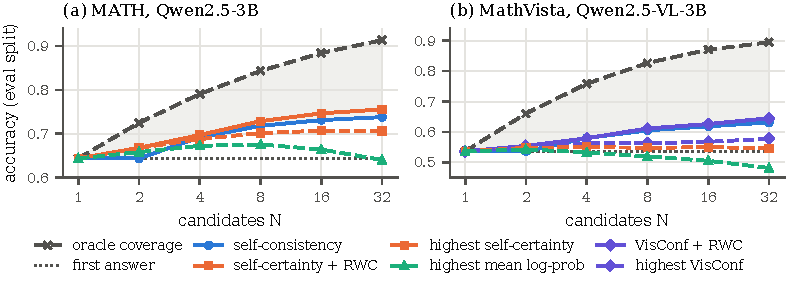
\includegraphics[width=\linewidth]{fig_task3_scaling.pdf}
  \caption{\textbf{Accuracy against the number of candidates} on the 800 evaluation questions. The dashed grey line is oracle coverage (some candidate is correct). The shaded band between it and self-consistency is the share of questions where a correct answer was sampled but not selected. Solid coloured lines aggregate by votes (self-consistency, RWC); dashed coloured lines pick the single highest-scoring rollout. Source: \file{offline\_summary.csv}.}
  \label{fig:task3scaling}
\end{figure}

Repeated sampling creates a large opportunity (Figure~\ref{fig:task3scaling}). From one rollout to 32, oracle coverage, the chance that some rollout is correct, rises from 64.4\% to 91.4\% on MATH and from 53.6\% to 89.5\% on MathVista, while self-consistency reaches only 73.8\% and 63.1\%. The remaining failures are of two kinds. Questions with no correct rollout fall to 8.6\% and 10.5\% at $N=32$, while questions where a correct rollout was sampled but not chosen grow to 17.6\% and 26.4\%. The second kind overtakes the first between $N=8$ and 16 on MATH and between 4 and 8 on MathVista, after which selection rather than sampling limits accuracy. The reason lies in where the new coverage comes from. Grouping questions by the share of their 32 rollouts that are correct (a retrospective view using gold labels), 58\% of the MATH coverage gain and 47\% of the MathVista gain come from questions where at most a quarter of rollouts are correct. In these the correct answer is a minority by construction, and self-consistency barely moves (MATH 11.4\% to 13.3\%) or even falls (MathVista 14.1\% to 5.7\%).

Quality scores help only when they weight a vote rather than pick a winner, and the gap grows with $N$ (Figure~\ref{fig:task3scaling} and Table~\ref{tab:task3methods} in the appendix). With the score fixed, RWC beats highest-score selection at every $N\geq4$ on both datasets, by 0.9 to 4.9 points for self-certainty on MATH and by up to 10.3 points for visual engagement on MathVista, every interval excluding zero. Highest-score rules flatten or even decline as $N$ grows, and highest mean log-probability ends below the first answer on both datasets, because more candidates give a single-score rule more chances to meet a confidently wrong outlier. At $N=32$ it picks an answer that no other rollout supports 13.1\% of the time on MATH (self-consistency: 0.1\%) and NO\_ANSWER, mostly from rollouts looping until the token cap, 14.4\% of the time. With the aggregation fixed, the choice of score matters mainly when the score acts alone. Under highest-score selection, self-certainty beats mean log-probability by 6.6 points on MATH and VisConf beats self-certainty by 3.1 on MathVista, but under RWC these differences shrink below 1 point and lose significance, since an answer group's summed rank weights are dominated by its size. Only self-certainty with RWC on MATH beats plain voting significantly, by 1.8 points. On MathVista no rule is distinguishable from self-consistency at $N=32$, including VisConf with RWC ($+1.4$), which also needs attention maps from every layer for every token, a cost the token count leaves out.

How well each score separates correct from incorrect rollouts within a question explains this behaviour. Comparing the correctness of each question's 8 top-scored and 8 bottom-scored rollouts at $N=32$ (questions with mixed outcomes), self-certainty separates them more strongly than log-probability on MATH (20.4 against 13.4 points), matching their order as selectors. On MathVista every single signal is weak ($L$ 2.0, $K$ 4.4, $V$ 4.8 and VisConf 9.3 points), and length confounds them. Correct rollouts are shorter than incorrect ones (by 87 tokens on MATH and 80 on MathVista), yet within-question Spearman correlations with length are positive for $L$ ($+0.22$, $+0.33$) and, on MathVista, for $K$ ($+0.35$), which pushes these scores towards wrong answers. Visual engagement is the clearest case, with a correlation of $-0.69$: as a rollout grows, attention shifts from the image to the generated text, so a high image share mostly marks a short rollout, and ranking by shortness alone separates the quartiles about as well (5.0 points). Within rollouts, confidence and visual engagement are negatively correlated (per-question mean Pearson correlation $-0.21$, interquartile range $-0.30$ to $-0.09$), so confident tokens tend to attend less to the image. Fusing the two per token, $Z^{\mathrm{token}}_i=\frac{1}{T_i}\sum_tc_{i,t}v_{i,t}$, differs from VisConf by exactly $\mathrm{Cov}_t(c_{i,t},v_{i,t})$, which is small (mean $-0.0022$), and never changes accuracy significantly under either rule. These are attention-share associations; without an image intervention they cannot show that the selected answers use the image.

A small live experiment asks a related question with fresh generations. On 50 MATH questions, Qwen2.5-3B-Instruct spends a 3,072-token output allowance in three ways: one long response, three parallel 1,024-token responses combined by vote, or one response followed by a self-review and revision (Table~\ref{tab:task3live} in the appendix). Their accuracies, 0.58, 0.56 and 0.62, lie within six points of each other, and no paired difference excludes zero; refinement against parallel only touches zero and rests on three questions. The mechanics are clearer than the accuracies. 26 of 150 parallel calls hit their cap, and in 9 questions the vote fell on NO\_ANSWER, including all three questions where refinement beat parallel. The revision changed the initial answer in 8 questions, each of whose initial responses had been cut off without an answer (2 became correct). In the 42 questions where the initial response did contain an answer, the revision never changed it, and accuracy stays at 69.0\%: revision completed truncated work but never fixed an existing answer. Equal caps also do not mean equal spend: the single response used 22\% of its allowance, and actual output differs 2.7 times across strategies. At this scale, cost and truncation separate breadth from reconsideration; accuracy does not.

\begin{figure}[t]
  \centering
  \begin{minipage}[b]{0.50\linewidth}
    \centering
    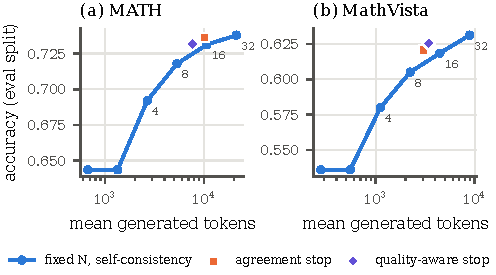
\includegraphics[width=\linewidth]{fig_task3_adaptive.pdf}
  \end{minipage}\hfill
  \begin{minipage}[b]{0.48\linewidth}
    \footnotesize
    \setlength{\tabcolsep}{2.4pt}
    \begin{tabular}{lccc}
      \toprule
      Policy & acc. $-$ fixed 32 & tokens & stop at 4 \\
      \midrule
      \multicolumn{4}{l}{\emph{MATH} (fixed 32: 73.8\%, 21,347 tokens)} \\
      agree, $\tau{=}.625$ & $-0.15$ \ci{$-0.50$}{0.16} & 47\% & 66\% \\
      quality, $\tau{=}.5$ & $-0.61$ \ci{$-1.20$}{$-0.06$} & 36\% & 76\% \\
      \multicolumn{4}{l}{\emph{MathVista} (fixed 32: 63.1\%, 8,898 tokens)} \\
      agree, $\tau{=}.5$ & $-1.05$ \ci{$-2.08$}{0.13} & 34\% & 75\% \\
      quality, $\tau{=}.5$ & $-0.58$ \ci{$-1.44$}{0.40} & 39\% & 68\% \\
      \bottomrule
    \end{tabular}
    \vspace{6pt}
  \end{minipage}
  \caption{\textbf{Adaptive stopping on the evaluation split.} Left: accuracy against mean generated tokens for fixed-$N$ self-consistency (labelled by $N$) and the two controllers chosen on development data. Right: accuracy change in pp against fixed $N=32$ with 95\% interval, token cost as a share of fixed 32, and share of question orders stopped at the first check ($n=4$). Both quality controllers selected $\gamma=0$. Sources: \file{adaptive\_eval.csv}, \file{adaptive\_bootstrap.csv}, \file{adaptive\_selected.json}.}
  \label{fig:task3adaptive}
\end{figure}

The cheapest gain comes from not sampling more than needed. Two controllers reveal rollouts in order and stop at $n\in\{4,8,16\}$ once a non-missing answer holds a fraction $\tau$ of the votes; the quality-aware one also requires the RWC winner to agree, by a margin $\gamma$. Both return the current self-consistency answer, so they differ only in when they stop. Development data selected the cheapest $\tau$ and $\gamma$ within one point of fixed-32 accuracy, and both quality controllers chose $\gamma=0$, which reduces the extra condition to agreement between the self-consistency and RWC winners. On held-out questions all four controllers keep most of fixed-32 accuracy at a third to a half of its cost, 0.7 to 1.3 points above fixed-$N$ voting interpolated to the same mean cost (Figure~\ref{fig:task3adaptive}). The development tolerance did not always hold: the MATH quality controller is significantly below fixed 32 yet within one point ($-0.61$), and the MathVista agreement controller's $-1.05$ exceeds it, with an interval spanning both zero and $-1$. On MATH the quality controller is the cheaper one only because development allowed it a lower $\tau$ (0.5 against 0.625); on MathVista, at equal $\tau$, its extra condition makes it stop later and cost more. Stopping follows agreement in the full pool as intended: questions whose 32 rollouts all agree stop after about 4, while those with a plurality share below a quarter use 24 to 31 rollouts on average. Most wrong early stops cost nothing relative to fixed 32, since only 8 to 18\% of the 660 to 1,966 wrong early stops per controller would have been answered correctly by consuming all 32. A deployed controller would also save the prefill and scoring of rollouts it never generates, which the token count leaves out.
